\subsection{Aufbau der BTS}

Der letztendliche Aufbau der \gls{bts} im finalen Zustand ist in Abbildung \ref{fig:ClassDiagramBTS} ersichtlich. Grunds�tzlich befindet sich das ViewModel in der Klasse \inline{MainViewModel} und wird von der Klasse \inline{Order} unterst�tzt. Der View befindet sich in der dazugeh�rigen Klasse \inline{MainWindow} und alle restlichen Klassen stellen das Model dar.

\begin{figure}[h]
	\centering
		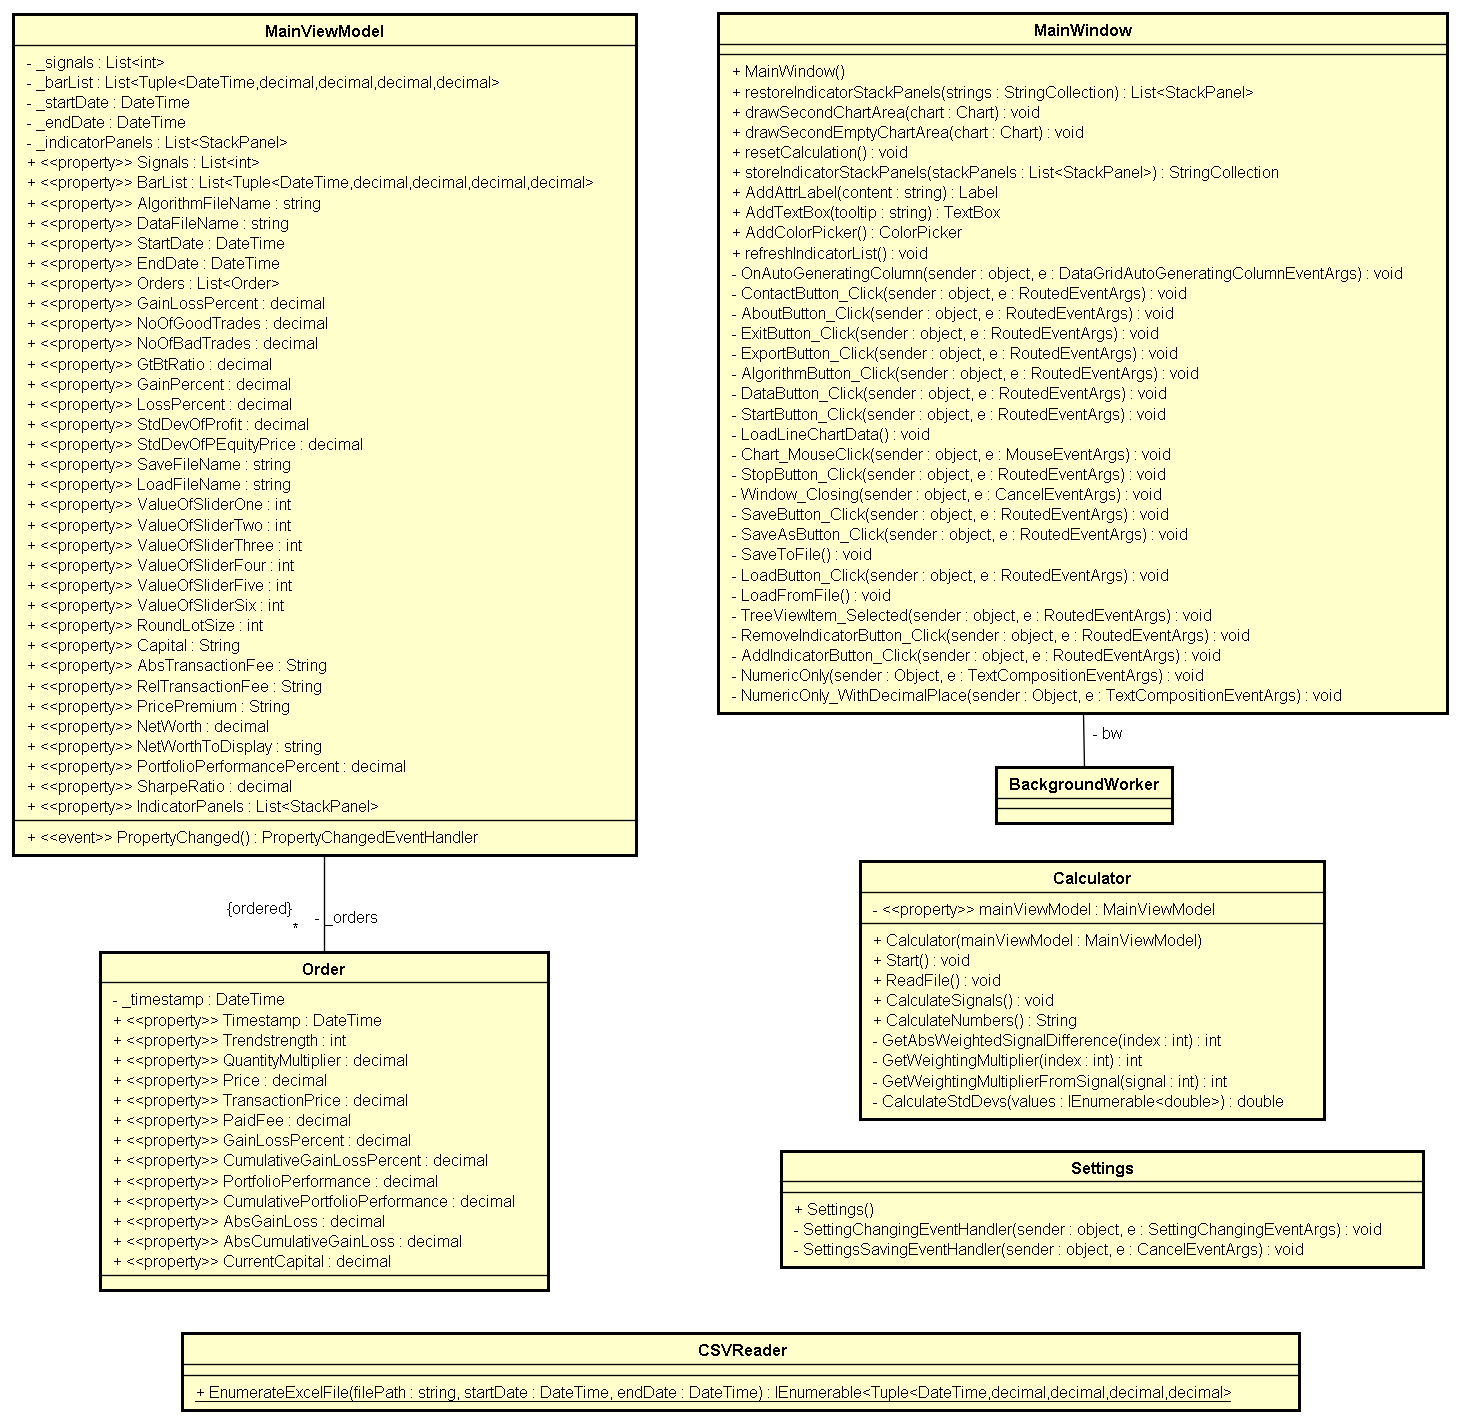
\includegraphics[width=1.00\textwidth]{graphics/ergebnis/Noctua_BTS_ClassDiagram.png}
	\caption{Klassendiagram der \gls{bts}}
	\label{fig:ClassDiagramBTS}
\end{figure}

Das \inline{MainWindow} der \gls{bts} stellt zusammen mit der dazugeh�rigen \gls{xaml}-Datei den View der Applikation dar, es besitzt allerdings auch noch ein wenig mehr Zusatzfunktionalit�t. Es behandelt die Events aller Button-Klicks, ist f�r den Aufbau des Charts zust�ndig und beinhaltet alle weiteren Funktionalit�ten der \gls{gui}-Elemente. Deshalb besitzt es nat�rlich auch die Codest�cke f�r das Speichern, Laden und Exportieren der Performancedaten, den Aufbau und die Verwaltung der Charts und Indikatoren und vieles mehr. Der \inline{BackgroundWorker} wird hierbei dazu benutzt, um die Berechnungen des \inline{Calculator}s in einen \inline{Thread} auszulagern.\\
\\
Das \inline{MainViewModel} der \gls{bts} ist eine sehr einfache Form des ViewModels, indem es lediglich alle f�r die \gls{gui} relevanten Daten speichert. Welche das genau sind, kann ebenfalls der Abbildung \ref{fig:ClassDiagramBTS} entnommen werden. Dazu ben�tzt es die Technologie des Data Bindings auf Properties, die bei einer Ver�nderung �ber Events direkt die neuen Daten im View anzeigen. F�r die Darstellung des \inline{DataGrid}s auf dem Orders-Tab der \gls{bts} wird zus�tzlich noch die Klasse \inline{Order} bzw. eine Liste aus \inline{Order}-Objekten im ViewModel gespeichert, die selbst auch wieder Properties besitzen.\\
\\
Die wohl wichtigste Klasse des Models ist der \inline{Calculator}. Hier werden alle Berechnungen zur Erhebung von Performancedaten durchgef�hrt. Er hat also auch direkt Zugriff auf das ViewModel und setzt dort die errechneten Daten, die daraufhin in der \gls{gui} angezeigt werden. Weiters ben�tzt der \inline{Calculator} den \inline{CSVReader}, um die historischen Aktien-Preisdaten aus dem gew�hlten \gls{csv}-File auszulesen und besitzt auch selber entsprechenden Code, um den gew�hlten Algorithmus in Form einer \gls{dll}-Datei einzulesen und zu invokieren. Innerhalb aller Berechnungen des \inline{Calculator}s werden Bars immer in der Form \inline{List<Tuple<DateTime, decimal, decimal, decimal, decimal>>} gespeichert. Zu guter Letzt gibt es da nun noch die \inline{Settings}-Klasse. Diese wird von Microsoft Visual Studio automatisch generiert und unterts�tzt den Programmierer bei der Arbeit mit Anwendungskonfigura\-tionsdateien (siehe \ref{akd} "`Anwendungskonfigurationsdateien"').